% !TEX TS-program = xelatex
% !BIB program = bibtex
% !TeX spellcheck = ru_RU

% About magic macroses see also
% https://tex.stackexchange.com/questions/78101/

% По умолчанию используется шрифт 14 размера. Если нужен 12-й шрифт, уберите опцию [14pt]
\documentclass[14pt, russian]{matmex-diploma-custom}

% !TeX spellcheck = ru_RU
% !TEX root = vkr.tex
% Опциональные добавления используемых пакетов. Вполне может быть, что они вам не понадобятся, но в шаблоне приведены примеры их использования.
\usepackage{tikz} % Мощный пакет для создание рисунков, однако может очень сильно замедлять компиляцию
\usetikzlibrary{decorations.pathreplacing,calc,shapes,positioning,tikzmark}

% Библиотека для TikZ, которая генерирует отдельные файлы для каждого рисунка
% Позволяет ускорить компиляцию, однако имеет свои ограничения
% Например, ломает пример выделения кода в листинге из шаблона
% \usetikzlibrary{external}
% \tikzexternalize[prefix=figures/]

\newcounter{tmkcount}

\tikzset{
  use tikzmark/.style={
    remember picture,
    overlay,
    execute at end picture={
      \stepcounter{tmkcount}
    },
  },
  tikzmark suffix={-\thetmkcount}
}

\usepackage{booktabs} % Пакет для верстки "более книжных" таблиц, вполне годится для оформления результатов
% В шаблоне есть команда \multirowcell, которой нужен этот пакет.
\usepackage{multirow}
\usepackage{siunitx} % для таблиц с единицами измерений

\newcommand{\cd}[1]{\texttt{#1}}
\newcommand{\inbr}[1]{\left<#1\right>}

% Для названий стоит использовать \textsc{}
\newcommand{\OCaml}{\textsc{OCaml}}
\newcommand{\miniKanren}{\textsc{miniKanren}}
\newcommand{\BibTeX}{\textsc{BibTeX}}
\newcommand{\vsharp}{\textsc{V$\sharp$}}
\newcommand{\fsharp}{\textsc{F$\sharp$}}
\newcommand{\csharp}{\textsc{C$\sharp$}}
\newcommand{\GitHub}{\textsc{GitHub}}
\newcommand{\SMT}{\textsc{SMT}}

\newcolumntype{L}[1]{>{\raggedright\let\newline\\\arraybackslash\hspace{0pt}}m{#1}}
%\newcolumntype{C}[1]{>{\centering\let\newline\\\arraybackslash\hspace{0pt}}m{#1}}
\newcolumntype{R}[1]{>{\raggedleft\let\newline\\\arraybackslash\hspace{0pt}}m{#1}}

\usepackage{xcolor}

%  Команды и пакеты, не используемые в шаблоне, которые тем не менее могут быть полезными.

% \newcolumntype{Y}{>{\centering\arraybackslash}X}

% \usepackage{mathrsfs}

\lstdefinestyle{fsharp}{
  basicstyle=\small\ttfamily,
  keywordstyle=\color{blue},
  commentstyle=\color{lightblue},
  stringstyle=\color{red},
  numbers=left,
  numberstyle=\tiny\color{gray},
  stepnumber=1,
  numbersep=10pt,
  backgroundcolor=\color{white},
  showspaces=false,
  showstringspaces=false,
  showtabs=false,
  tabsize=2,
  breaklines=true,
  breakatwhitespace=false,
  morekeywords={async, let, rec, if, then, else, do, yield, return, use, match, with, function}
  literate={->}{{$\to$}}3 {==}{{$\equiv$}}1 {=/=}{{$\not\equiv$}}1 {|>}{{$\triangleright$}}3 {\\/}{{$\vee$}}2 {/\\}{{$\wedge$}}2 {>=}{{$\ge$}}1 {<=}{{$\le$}}
}


\usepackage{totcount}

\begin{document}
% TODO: Formatting
% !TeX spellcheck = ru_RU
% !TEX root = vkr.tex

%% Если что-то забыли, при компиляции будут ошибки Undefined control sequence \my@title@<что забыли>@ru
%% Если англоязычная титульная страница не нужна, то ее можно просто удалить.
\filltitle{ru}{
    %% Актуально только для курсовых/практик. ВКР защищаются не на кафедре а в ГЭК по направлению,
    %%   и к моменту защиты вы будете уже не в группе.
    chair              = {Кафедра системного программирования},
    group              = {22.Б07-мм},
    %
    %% Макрос filltitle ненавидит пустые строки, поэтому обязателен хотя бы символ комментария на строке
    %% Актуально всем.
    title              = {Реализация процедурной генерации интерьера комнат в 3D-игре на Unity},
    %
    %% Здесь указывается тип работы. Возможные значения:
    %%   production - производственная практика;
    %%   coursework - отчёт по курсовой работе;
    %%   practice - отчёт по учебной практике;
    %%   prediploma - отчёт по преддипломной практике;
    %%   master - ВКР магистра;
    %%   bachelor - ВКР бакалавра.
    type               = {practice},
    %
    %% Здесь указывается вид работы. От вида работы зависят критерии оценивания.
    %%   solution - <<Решение>>. Обучающемуся поручили найти способ решения проблемы в области разработки программного обеспечения или теоретической информатики с учётом набора ограничений.
    %%   experiment - <<Эксперимент>>. Обучающемуся поручили изучить возможности, достоинства и недостатки новой технологии, платформы, языка и т. д. на примере какой-то задачи.
    %%   production - <<Производственное задание>>. Автору поручили реализовать потенциально полезное программное обеспечение.
    %%   comparison - <<Сравнение>>. Обучающемуся поручили сравнить несколько существующих продуктов и/или подходов.
    %%   theoretical - <<Теоретическое исследование>>. Автору поручили доказать какое-то утверждение, исследовать свойства алгоритма и т.п., при этом не требуя написания кода.
    kind               = {production},
    %
    author             = {САВЕЛЬЕВА Полина Андреевна},
    %
    %% Актуально только для ВКР. Указывается код и название направления подготовки. Типичные примеры:
    %%   02.03.03 <<Математическое обеспечение и администрирование информационных систем>>
    %%   02.04.03 <<Математическое обеспечение и администрирование информационных систем>>
    %%   09.03.04 <<Программная инженерия>>
    %%   09.04.04 <<Программная инженерия>>
    %% Те, что с 03 в середине --- бакалавриат, с 04 --- магистратура.
    specialty          = {02.03.03 <<Математическое обеспечение и администрирование информационных систем>>},
    %
    %% Актуально только для ВКР. Указывается шифр и название образовательной программы. Типичные примеры:
    %%   СВ.5006.2017 <<Математическое обеспечение и администрирование информационных систем>>
    %%   СВ.5162.2020 <<Технологии программирования>>
    %%   СВ.5080.2017 <<Программная инженерия>>
    %%   ВМ.5665.2019 <<Математическое обеспечение и администрирование информационных систем>>
    %%   ВМ.5666.2019 <<Программная инженерия>>
    %% Шифр и название программы можно посмотреть в учебном плане, по которому вы учитесь.
    %% СВ.* --- бакалавриат, ВМ.* --- магистратура. В конце --- год поступления (не обязательно ваш, если вы были в академе/вылетали).
    programme          = {СВ.5006.2019 <<Математическое обеспечение и администрирование информационных систем>>},
    %
    %% Актуально только для ВКР, только для матобеса и только 2017-2018 годов поступления. Указывается профиль подготовки, на котором вы учитесь.
    %% Названия профилей можно найти в учебном плане в списке дисциплин по выбору. На каком именно вы, вам должны были сказать после второго курса (можно уточнить в студотделе).
    %% Вот возможные вариканты:
    %%   Математические основы информатики
    %%   Информационные системы и базы данных
    %%   Параллельное программирование
    %%   Системное программирование
    %%   Технология программирования
    %%   Администрирование информационных систем
    %%   Реинжиниринг программного обеспечения
    % profile            = {Системное программирование},
    %
    %% Актуально всем.
    %supervisorPosition = {проф. каф. СП, д.ф.-м.н., проф.}, % Терехов А.Н.
    supervisorPosition = {доцент кафедры системного программирования, к.т.н.}, % Григорьев С.В.
    supervisor         = {Ю.~В.~Литвинов},
    %
    %% Актуально только для практик и курсовых. Если консультанта нет, закомментировать или удалить вовсе.
    consultantPosition = {студент 3-го курса СПбГУ,},
    consultant         = {Р.~А.~Береснёв},
    %
    %% Актуально только для ВКР.
    reviewerPosition   = {должность ООО <<Место работы>> степень},
    reviewer           = {Р.~Р.~Рецензент},
}

% \filltitle{en}{
%     chair              = {Advisor's chair},
%     group              = {ХХ.BХХ-mm},
%     title              = {Template for SPbU qualification works},
%     type               = {practice},
%     author             = {FirstName Surname},
%     %
%     %% Possible choices:
%     %%   02.03.03 <<Software and Administration of Information Systems>>
%     %%   02.04.03 <<Software and Administration of Information Systems>>
%     %%   09.03.04 <<Software Engineering>>
%     %%   09.04.04 <<Software Engineering>>
%     %% Те, что с 03 в середине --- бакалавриат, с 04 --- магистратура.
%     specialty          = {02.03.03 ``Software and Administration of Information Systems''},
%     %
%     %% Possible choices:
%     %%   СВ.5006.2017 <<Software and Administration of Information Systems>>
%     %%   СВ.5162.2020 <<Programming Technologies>>
%     %%   СВ.5080.2017 <<Software Engineering>>
%     %%   ВМ.5665.2019 <<Software and Administration of Information Systems>>
%     %%   ВМ.5666.2019 <<Software Engineering>>
%     programme          = {СВ.5006.2019 ``Software and Administration of Information Systems''},
%     %
%     %% Possible choices:
%     %%   Mathematical Foundations of Informatics
%     %%   Information Systems and Databases
%     %%   Parallel Programming
%     %%   System Programming
%     %%   Programming Technology
%     %%   Information Systems Administration
%     %%   Software Reengineering
%     % profile            = {Software Engineering},
%     %
%     %% Note that common title translations are:
%     %%   кандидат наук --- C.Sc. (NOT Ph.D.)
%     %%   доктор ... наук --- Sc.D.
%     %%   доцент --- docent (NOT assistant/associate prof.)
%     %%   профессор --- prof.
%     supervisorPosition = {Sc.D, prof.},
%     supervisor         = {S.S. Supervisor},
%     %
%     consultantPosition = {position at ``Company'', degree if present},
%     consultant         = {C.C. Consultant},
%     %
%     reviewerPosition   = {position at ``Company'', degree if present},
%     reviewer           = {R.R. Reviewer},
% }

\maketitle
\setcounter{tocdepth}{3}
\tableofcontents

% \begin{abstract}
%   В курсаче не нужен
% \end{abstract}

% !TeX spellcheck = ru_RU
% !TEX root = vkr.tex

\section{Введение}
\thispagestyle{withCompileDate}

Time Reactor\footnote{https://github.com/RuslanBeresnev/Time-Reactor-Game (дата обращения: \DTMdate{2024-01-2}).} --- это научно-фантастическая 3D игра на \textit{Unity}, разработанная студентом СПбГУ Русланом Бересневым в качестве семестровой практики. К задачам по расширению игрового мира Time Reactor относится реализация \textit{процедурной генерации} интерьера комнат.  Выполнение этой задач предоставляет возможность не только изучить основы Unity Engine и процедурной генерации, но и добавить новые игровые механики в перспективный проект.

Основным местом действия игры является \enquote{бесконечная} лестница. На ее этажах случайным образом располагаются помещения одного из трех типов: лаборатория, компьютерный центр и склад. Игроку предстоит посетить около сотни подобных помещений прежде, чем он доберется до финальной комнаты. Ручное заполнение подобных локаций представляется объемной задачей с существенными временными затратами \cite{short2017procedural}. В качестве альтернативного подхода по созданию большого количества разнообразных интерьеров используются методы процедурной генерации.
    
Под процедурной генерацией контента (Procedural Content Ge\-ne\-ra\-ti\-on, \textit{PCG}) понимается наполнение игрового мира с помощью алгоритмов \cite{article}. Методы PCG широко используются при разработке игр \cite{dahren2021usage} --- от генерации целых уровней в Spelunky (Mossmouth 2009) и планет
в No Man’s Sky (Hello Games 2016) до характеров персонажей и сюжетов в RimWorld (Ludeon Studios 2013). В первой главе книги \enquote{Procedural generation in game design} Tanya Short и Tarn Adams перечисляют ряд причин, побуждающих разработчиков использовать методы процедурной генерации в своих проектах:
\begin{itemize}
    \item создание разнообразного наполнения в масштабах, недостижимых вручную;
    \item отсутствует необходимость в хранении сгенерированных данных;
    \item грамотно спроектированный алгоритм позволит сэкономить время на ручном заполнении комнат;
    \item повторное использование генераторов.
\end{itemize}

В свою очередь, \textit{процедурная генерация помещений} направлена на создание виртуальной среды, приближенной к реальной, с помощью алгоритмов PCG. Процедурно генерируемое помещение строится из описания объектов, характерных для данного пространства, и связей между ними. К последнему можно отнести \textit{иерархические паттерны} (посуда на кухне располагается строго на полках, стулья в кабинете за письменным столом) и функциональные требования (экран телевизора находится в зоне видимости и не заставлен другими предметами).

Для придания большей реалистичности игровому миру система генерации должна отвечать и другим требованиям. В частности, активировать  алгоритм следует в наиболее подходящий момент, например, при попадании комнаты в зону видимости. Процесс расстановки следует проводить достаточно быстро, чтобы избежать ситуаций, когда мебель появляется на глазах у игрока. Также немаловажно сохранить интерьер неизменным при каждом следующем посещении.

Таким образом, необходимо не только реализовать алгоритм для процедурной генерации реалистичного интерьера комнат, но и обеспечить его эффективную интеграцию с остальными игровыми процессами, а также неизменность результата при многократном вызове.
% !TeX spellcheck = ru_RU
% !TEX root = vkr.tex

\section{Постановка задачи}

Целью данной работы является реализация процедурной генерации интерьера комнат в игре Time Reactor на Unity. Для её выполнения были поставлены следующие задачи.

\begin{itemize}
    \item Реализация .NET библиотеки для процедурной генерации интерьера комнат.
    \item Реализация процедурной генерации интерьера комнат в игре Time
    Reactor на Unity с использованием разработанной библиотеки.
    \item Проведение апробации среди заинтересованных игроков.
\end{itemize}
% !TeX spellcheck = ru_RU
% !TEX root = vkr.tex

\section{Обзор}

В данном разделе представлен обзор существующих методов и технологий, связанных с процедурной генерацией интерьера. В частности, будут рассмотрены агентный и основанный на правилах подходы и некоторые особенности Unity проекта.


\subsection{Существующие решения}

Исследователи в работе \enquote{Recent Advances in Procedural Generation of Buildings: From Diversity to Integration} проанализировали существующие подходы к процедурной генерации интерьеров зданий. Около 65\% решений используют методы, \textit{основанные на правилах} (rule-based approach), около 20\% --- машинное обучение и менее 10\% --- \textit{агентный подход} (agents approach). Наименьшее распространение получил способ \enquote{замены} (substitution approach), включающий в себя L-системы и грамматики форм. Системы, унифицирующие машинное обучение, вопреки своей растущей популярности \cite{kutzias2023recent}, имеют существенный порог вхождения и требуют значительных временных трат \cite{kan2021automatic,balint2019generalized}. Таким образом, для решения поставленной задачи предпочтительнее использовать агентный или основанный на правилах подход.

\subsubsection{Агентный подход}

Исследователи под руководством Germer \cite{germer2009procedural} представили систему расстановки мебели, работающую в режиме реального времени. В ней каждый предмет интерьера является автономным агентом и обладает способностью к перемещению и оценке собственного положения. По словам авторов, у системы имеются некоторые недостатки. Например, нельзя явно указать телевизору на необходимость размещения на стене прямо напротив дивана или задать другие сложные иерархические зависимости. А в условиях быстрого перемещения пользователя система не успевает заполнить достаточное количество комнат.

\begin{figure}
  \centering
  \begin{minipage}{0.45\textwidth}
    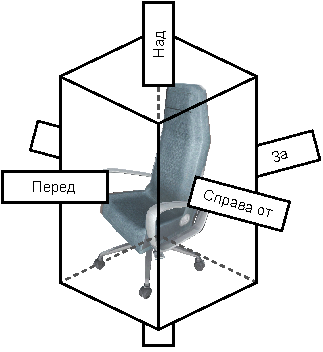
\includegraphics[width=0.8\textwidth]{matmex-diploma-template-master/figures/collider.pdf}
    \caption{Ограничительная рамка вокруг стула разделяет пространство вокруг на шесть зон}
    \label{fig:collider}
  \end{minipage}
  \hfill
  \begin{minipage}{0.45\textwidth}
    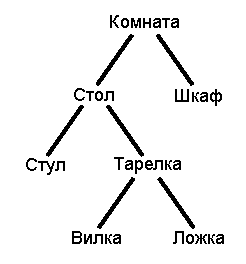
\includegraphics[width=0.8\textwidth]{matmex-diploma-template-master/figures/child_parent_relationship.pdf}
    \caption{Иерархическое представление комнаты}
    \label{fig:room_relationship}
  \end{minipage}
\end{figure}

Также в работе уделяется внимание представлению генерируемых объектов в виде упрощенных фигур. Исследователи пришли к выводу, что прямоугольный параллелепипед является хорошим приближением для многих объектов мебели. В таком представлении каждый предмет имеет ровно шесть граней, что сводит всевозможные случаи расстановки объектов к простым \enquote{перед}, \enquote{за}, \enquote{справа от} и т.~д (рис. \ref{fig:collider}). Наряду с этим авторы рассматривают концепцию детско-родительских отношений между предметами мебели, на вершине которой располагается вся декорируемая комната (рис. \ref{fig:room_relationship}).

\subsubsection{Основанный на правилах подход}

Идеи представления объектов, упомянутые выше, прослеживаются в работе \cite{lidberg2020hierarchical}. Условно их систему можно разделить на две составляющее: входные данные для генерации и сам алгоритм расстановки.

Входные данные определяются таблицей, содержащей сведения о всевозможных предметах мебели и их характеристиках.
Каждой строке соответствуют правила размещения объекта, вероятность его появления в различных пространствах, список предметов, которые он способен породить, и информация о том, является ли объект листовым, т.~e существующем исключительно по запросу родительского объекта. В свою очередь, алгоритм выражается в последовательности из шести шагов: инициализация генератора, выбор объекта, размещение и поиск свободного пространства, размещение листовых предметов и рекурсивный переход к заполнению дочерних пространств. В случае неудачи на некоторых шагах алгоритм способен вернуться на несколько итераций назад и повторить действия, пока положительный ответ не будет получен. Такое поведение может привести к неразрешимым сценариям, при которых время работы алгоритма окажется существенным, но в конечном итоге результат обещает быть более предсказуемым. 

После проведения независимого оценивания стало понятно --- система более чем способна генерировать реалистичные интерьеры. Участникам опроса до конца не сообщалось о целях его проведения, и многие из были уверены, что помогают человеку-дизайнеру подобрать лучшее интерьерное решение.

\subsection{Особенности Unity проекта}

Как было упомянуто раннее, Time Reactor --- это игра, созданная с использованием игрового движка Unity. До этого времени этажи заполнялись уже готовыми экземплярами комнат --- по одному на каждый тип помещения. Задача процедурной генерации интерьера, в свою очередь, заключалась именно в заполнении пустых версий этих комнат без изменения их размера и пропорций. В ином случае следует говорить о \textit{процедурно генерируемом экстерьере}.

Специфика Unity Engine позволяет использовать в игровых скриптах язык семейства .NET --- C\#. Это делает возможным интеграцию в проект библиотек на другом функциональном языке .NET --- F\#. Такой подход позволил отделить генератор от игры и открыл новые перспективы для использования алгоритма в других проектах.  

\subsection{Генератор псевдослучайных чисел}

Генератор псевдослучайных чисел решает проблему сохранения интерьера комнаты при ее повторном посещении. При инициализации на вход генератору поступает число, называемое \textit{random seed} или просто \textit{seed}. Одинаковые входные значения seed гарантируют одну и ту же последовательность чисел, выдаваемых генератором, при каждом запуске программы. 

В качестве псевдослучайного генератора в проекте используется экземпляр класса \texttt{Random} из пространства имен \texttt{System}. Входными данными для него служит номер этажа --- уникальное число, характеризующее каждую из комнат.

Вышесказанное совсем не означает, что помещения обязаны оставаться неизменными и после смерти игрока. Предположим, на третьем этаже в двух различных играх расположилось складское помещение. Интерьер в них будет идентичным --- генератор в обоих случаях задавался цифрой \enquote{3}. Для добавления большей вариативности в интерьерах перед процессом генерации данные для размещения перемешиваются. Схожая система уже используется в Time Reactor при расстановке врагов.
 
% !TeX spellcheck = ru_RU
% !TEX root = vkr.tex

\section{Реализация}

В данном разделе представлены детали реализации алгоритма по генерации интерьера с учетом методов и технологий, рассмотренных в обзорной части. В частности, ниже представлены: подробное объяснения алгоритма PCG, архитектура библиотеки и тонкости ее интеграции с Unity проектом.

\subsection{Разделение комнаты на ячейки}

Перед процессом генерации помещение разделяется на клетки или \textit{ячейки}. Количество ячеек по вертикали и горизонтали в точности совпадает с измерениями комнаты: шириной и высотой. Ячейка определяет минимально возможную единицу комнаты для расстановки в ней мебели. Каждая ячейка имеет индекс по строке и столбцу на комнатной \textit{решетке}, а также текущее состояние или \textit{статус}. К ним относятся, например, \texttt{Occupied} и \texttt{NonOccupied}, обозначающие доступна ли рассматриваемая ячейка для размещения или нет. Стоит заметить, что координаты ячеек показывают расположение объектов на локальной сетке относительно друг друга и их показатели должны быть скорректированы для совпадения с координатной системой игры.

\subsection{Входные данные}
Входными данными для алгоритма является \textit{таблица объектов}, которые необходимо разместить, и их характеристиками (рис. \ref{fig:data_table}). Строки таблицы или \texttt{DataTable} имеют следующую структуру.

\begin{enumerate}

    \item \textbf{Имя объекта}. Имя объекта играет роль маркера и помогает визуально отличить объекты в таблице и позже в Unity. 

    \item \textbf{Представители объекта}. Представителем является любая разновидность объекта, разделяющая его свойства. Например, объект с именем \enquote{стул} может иметь таких представителей как \enquote{синий стул} и \enquote{обеденный стул}. Каждый представитель определяется дополнительными параметрами: количество свободных ячеек справа от него, слева, спереди и сзади. Как следует из названия, свободные ячейки контролируют пространство вокруг объекта. Это также позволяет определить объекты, размеры которых превышают одну условную единицу.

    \item \textbf{Правила размещения} указывают на требования к размещению объекта. Правила описывают, является ли объект дочерним (\texttt{Leaf}) или нет (\texttt{Node}). В последнем случае положение объекта задается относительно всей комнаты, в случае \texttt{Leaf} объектов --- относительно родителя.

    \item \textbf{Дочерняя таблица}. В дочерней таблице представлена информация о предметах, которые может породить рядом с собой исходный объект. Структурно дочерняя таблица --- это экземпляр рассматриваемой \texttt{DataTable}. 
    
\end{enumerate}

\begin{figure}
    \centering
    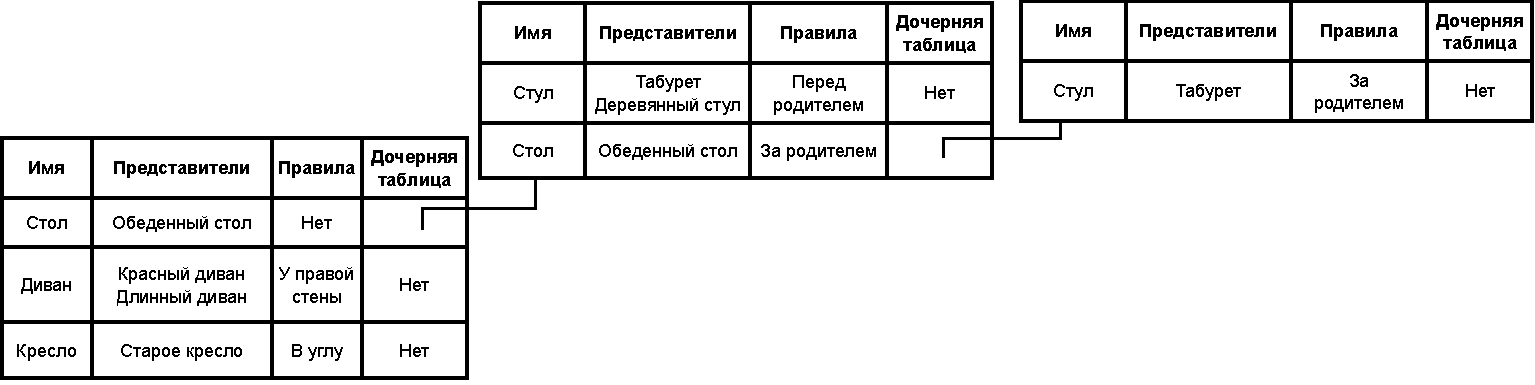
\includegraphics[width=\textwidth]{matmex-diploma-template-master/figures/data_table.pdf}
    \caption{Многоуровневая таблица объектов для размещения}
    \label{fig:data_table}
\end{figure}

\subsection{Алгоритм генерации интерьера}
Алгоритм генерации интерьера схож с рассмотренным в обзорной части, однако имеет ряд существенных отличий. Например, в целях уменьшения времени генерации объекты не могут быть удалены после размещения. Ниже приведено подробное описание искомого алгоритма. 

\begin{figure}
    \centering
    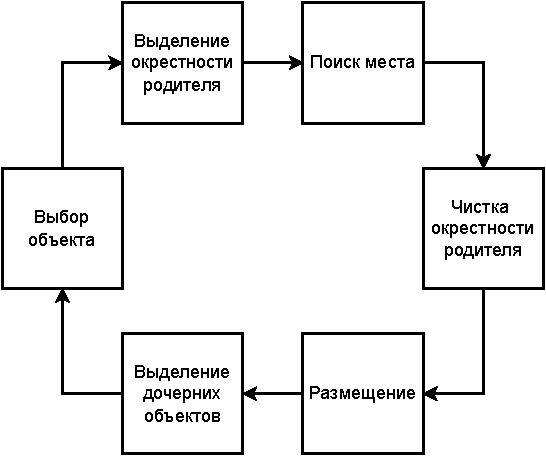
\includegraphics[width=0.4\textwidth]{matmex-diploma-template-master/figures/pcg.pdf}
    \caption{Последовательность шагов в алгоритме генерации интерьера}
    \label{fig:pcg}
\end{figure}

Шаги 1--6 повторяются, пока число объектов на сцене не достигло максимального или таблица объектов не пуста (рис. \ref{fig:pcg}).

\begin{enumerate}

    \item \textbf{Выбор объекта}. На данном этапе происходит выбор объекта для размещения с использованием генератора псевдослучайных чисел, который возвращает номер строки в таблице объектов и номер его представителя.

    \item \textbf{Выделение окрестности родителя}. Если выбранный предмет является дочерним, в зависимости от правил его размещения ячейки вокруг родительского объекта помечаются маркером \texttt{Oc\-cu\-pi\-ed\-For\-Chil\-dren}. На следующем шаге это позволит разместить дочерний объект рядом с родителем. 
    
    \item \textbf{Поиск места}. Поиск начинается с инициализации массива ячеек, соответствующих правилам размещения выбранного объекта. Например, если шкаф должен быть размещен у правой стены, то будут отобраны все незанятые клетки со статусом \texttt{Aga\-inst\-The\-Right\-Wall}. Из полученного массива случайным образом выбирается ячейка, которая должна стать центральной для объекта на сцене. В зависимости от наличия свободных ячеек вокруг объекта, на соответствие правилам  будет просмотрена и окрестность выбранной ячейки. Если окрестность не удовлетворяет правилам, искомая ячейка убирается из дальнейшего рассмотрения. Процесс будет повторятся, пока не будет найдена подходящая ячейка или массив не опустеет.  
    
    \item \textbf{Чистка окрестности родителя}. Если выбранный предмет является дочерним, то раннее помеченные \texttt{Oc\-cu\-pi\-ed\-For\-Chil\-dren} ячейки приобретают статус занятых. 
    
    \item \textbf{Размещение}. Если функция для поиска места вернула номер ячейки, то представитель объекта помещается в указанные координаты, а занятые ячейки (центральная и свободные ячейки указанные в правилах объекта) помечаются как \texttt{Occupied}. Иначе для выбранного представителя не существует свободного места и он убирается из рассмотрения, алгоритм возвращается к первому шагу. В случае, когда ни один представитель объекта не может разместиться --- из таблицы \enquote{удаляется} целая строка. Если окажется, что в первоначальной \texttt{DataTable} нет ни одной строки, процесс генерации останавливается.

    \item \textbf{Выделение дочерних объектов}. Если у размещенного объекта имеется таблица с дочерними объектами, алгоритм возвращается к первому шагу, принимая таблицу дочерних объектов за основную. Иначе возвращается к первому шагу с текущей \texttt{DataTable}. Когда таблица дочерних объектов становится пустой, алгоритм возвращается к случаю с родительской таблицей объектов. По этой причине на этапе смены таблиц информация о родителях и \texttt{CurrentDataTable} помещаются в стек.
    
\end{enumerate}

\begin{figure}
    \centering
    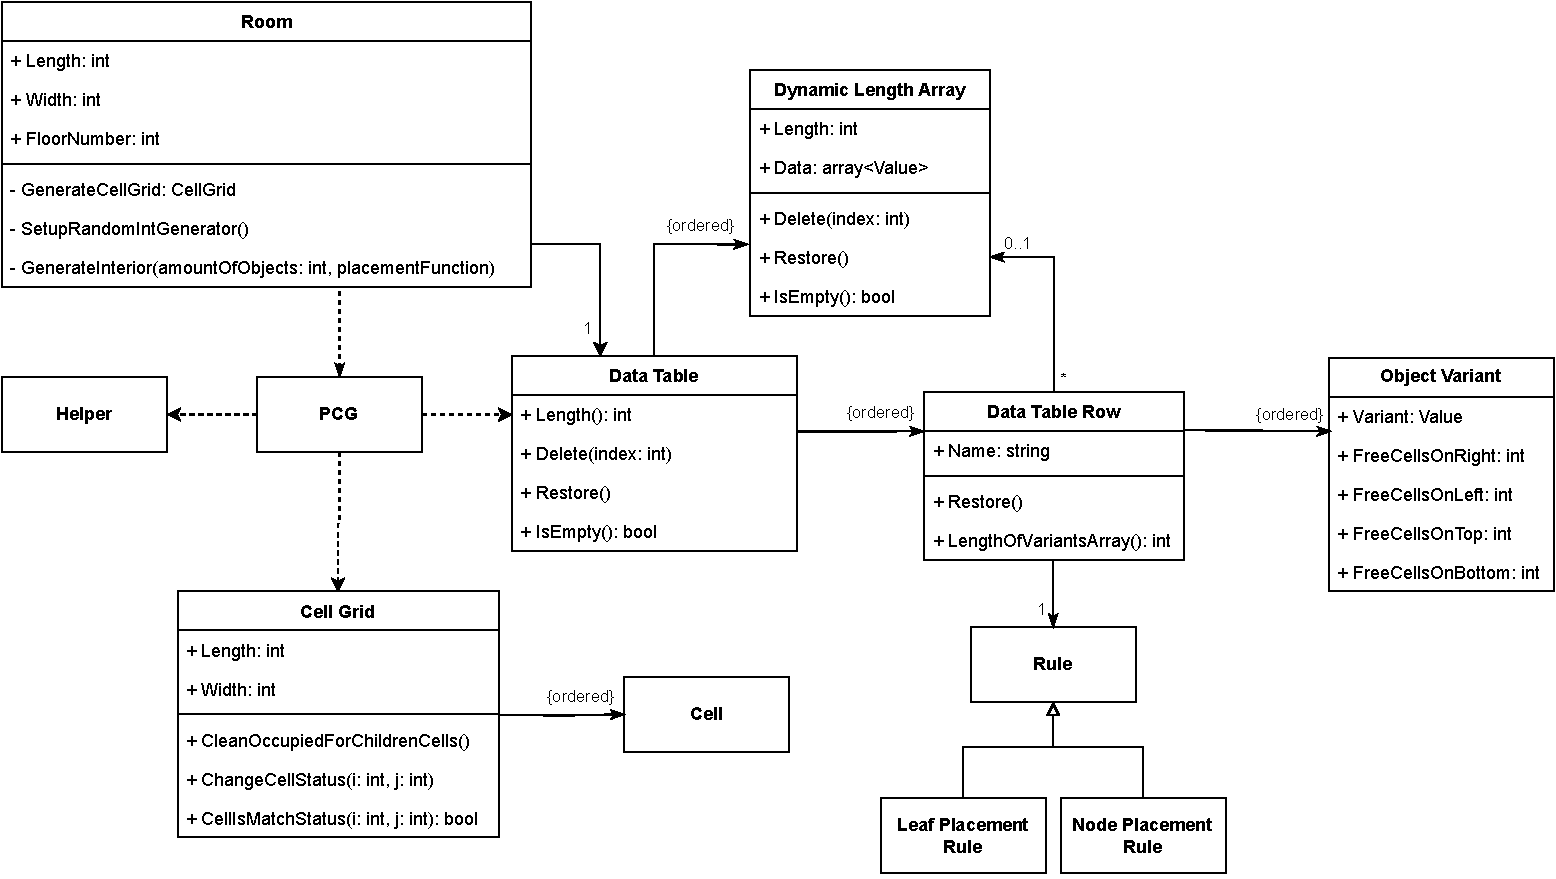
\includegraphics[width=\textwidth]{matmex-diploma-template-master/figures/uml.pdf}
    \caption{UML диаграмма классов библиотеки}
    \label{fig:uml}
\end{figure}

\subsection{Архитектура библиотеки}

Краткое описание модулей библиотеки представлено далее. Архитектура проекта представлена на UML диаграмме классов (диаг. \ref{fig:uml}). 

\begin{itemize}

    \item \textbf{Cell}. Данный модуль реализует ячейки, на которые разделяется комната, а также методы для проверки и изменения их состояний. Тип \texttt{Cell} представляет упомянутые раннее ячейки путем перечисления их состояний, например, \enquote{незанятая}, \enquote{угловая}, \enquote{зарезервированная для детей} и т.~д. В свою очередь, тип \texttt{CellGrid} инкапсулирует пространство для размещения в виде массива клеток. 
    
    \item \textbf{DataTable}. Модуль \texttt{DataTable} представляет инструменты для реализации входных данных алгоритма в виде таблиц, а также методы для удаления и восстановления ее строк. Типы, содержащиеся в модуле представлены далее.
        \begin{itemize}
            \item \texttt{LeafPlacementRule} и \texttt{NodePlacementRule} представляют возможные правила размещения для объектов. Тип \texttt{Rule} объединяет оба этих понятия.
    
            \item \texttt{ObjectVariant} описывает представителей объектов, дополненных размерами свободных ячеек вокруг них. Представитель может являться любым типом, совпадающим с сигнатурой функции размещения.
            
            \item \texttt{DataTableRow} представляет строку в таблице входных данных \texttt{DataTable}
        \end{itemize}
    
    \item \textbf{PCG} модуль содержит описанный алгоритм генерации.

    \begin{figure}
        \centering
        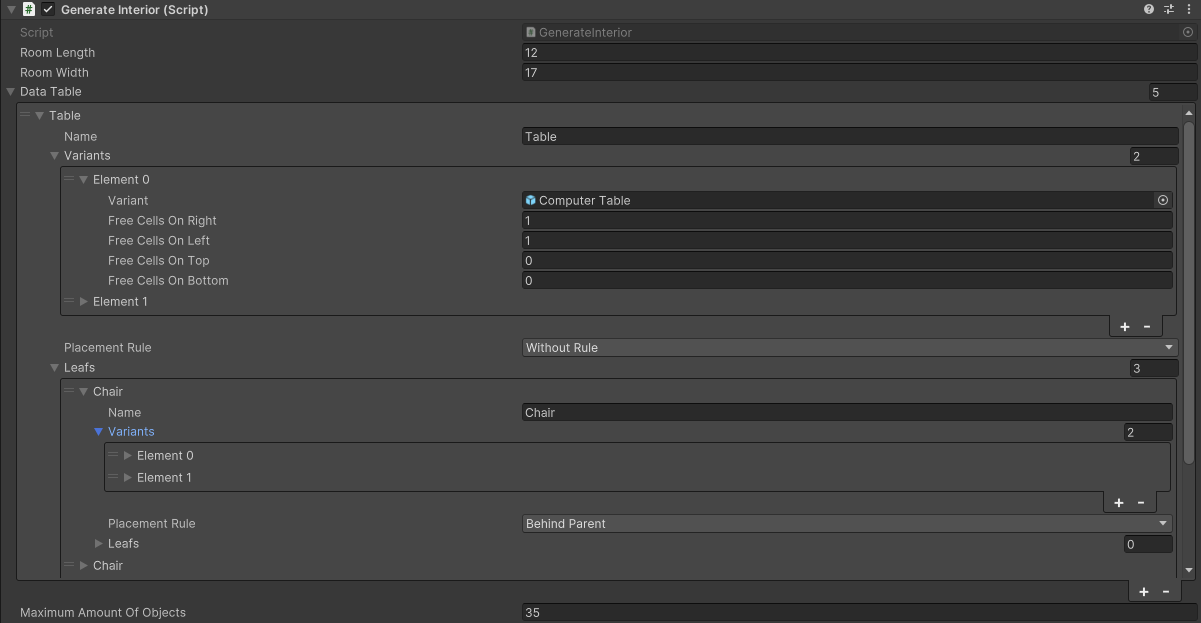
\includegraphics[width=\textwidth]{matmex-diploma-template-master/figures/inspector.png}
        \caption{Внешний вид панели Inspector в Unity}
        \label{fig:inspector}
    \end{figure}

    \item \textbf{Room} обобщает понятие комнаты. Модуль содержит информацию о ее размерах, номере этажа и таблице входных данных для декорирования. А также методы для разделения комнаты на ячейки, задания генератора псевдослучайных чисел и декорирования.
    
    \item \textbf{DynamicLengthArray} представляет массив переменной длины, используемый в представлении большинства структур библиотеки, в том числе \texttt{DataTable}. В отличие от честных динамических структур, изменение размера \texttt{DynamicLengthArray} не приводит к инициализации нового массива, а лишь сужает зону его видимости. Подобная механика, например, позволяет разным строкам \texttt{DataTable} ссылаться на одну дочернюю таблицу --- в конце итерации зона видимости вернется к прежнему значению и таблица \enquote{восстановится}. Другими словами, допустим, что объект \enquote{стол} породил все возможные дочерние объекты рядом. Как было описано раннее, при отсутствии свободного места, очередной листовой объект убирается из рассмотрения. Следовательно, дочерняя таблица окажется пустой, что станет проблемой для объекта \enquote{тумба}, ссылающегося на ту же дочернюю таблицу, что и \enquote{стол}. 
    
    \item \textbf{Helper} содержит вспомогательные функции.
    
\end{itemize}

Более подробно ознакомиться с API библиотеки можно на соответствующей странице GitHub Pages\footnote{https://polinasavelyeva.github.io/RoomInteriorGenerator/reference/index.html (дата обращения: \DTMdate{2023-12-16}).}.

Тестовое покрытие библиотеки составляет ~64\%. Такой процент был достигнут как с использованием ручных тестовых сценариев, так и при помощи тестирования на основе свойств.

\begin{figure}
    \centering
    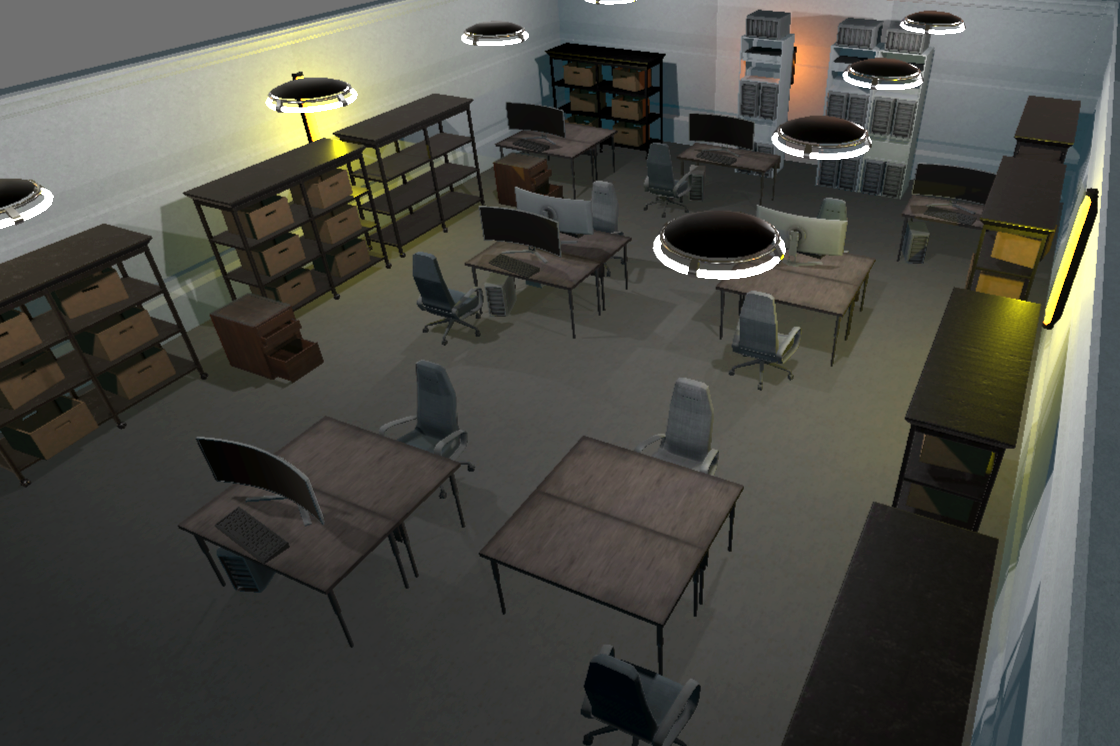
\includegraphics[width=0.45\textwidth]{matmex-diploma-template-master/figures/computing_center.png}
    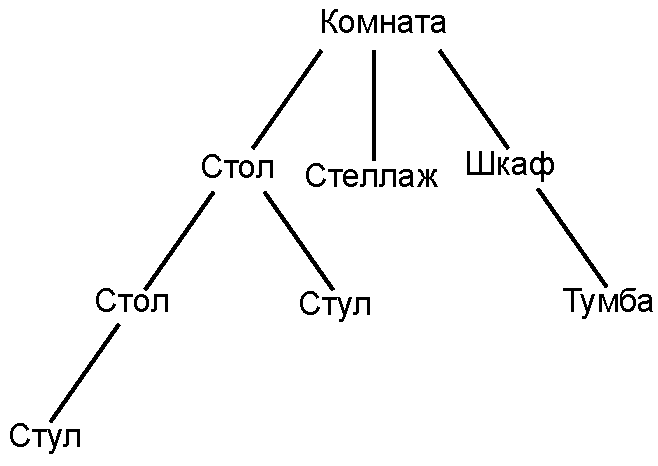
\includegraphics[width=0.45\textwidth]{matmex-diploma-template-master/figures/double_tables_tree.pdf}
    \caption{Процедурно заполненная комната с двойными столами (слева) и ее древовидное представление (справа)}
    \label{fig:double_table}
\end{figure}

\subsection{Реализация процедурной генерации в игре}

Логика генерации интерьера была реализована на панели Inspector (рис. \ref{fig:inspector}), содержащей свойства и компоненты объектов. Использование Inspector является распространенной практикой работы с Unity проектами, которая облегчает взаимодействие с игровыми скриптами и создает четкое разделение на программную и дизайнерскую составляющие. 

Каждое помещение заранее разделяется на зоны, необходимые к декорированию, такой прием позволяет, например, разместить предметы над и под складской лестницей. В левом верхнем углу каждой зоны размещается пустой игровой объект (которому \enquote{присваивают} скрипт генерации), являющийся началом координат для всех порожденных предметов мебели. Для получения ожидаемого результата следует дополнительно проверить, сходятся ли локальная координатная система области для декорирования и глобальная у игрового мира. 

Стоит обратить внимание и на то, в каком месте находится центр размещаемых объектов и на какой угол они изначально отклонены по каждой из осей. Некоторые объекты намеренно не соответствуют этим правилам, например, дочерний объект может быть заранее повернут на определенный угол --- такой прием позволил воссоздать сложную иерархическую структуру с двойными столами, представленную на рис. \ref{fig:double_table}. Примеры полученных комнат приведены на рис. \ref{fig:tech_warehouse}, \ref{fig:laboratory}.

\begin{figure}
    \centering
    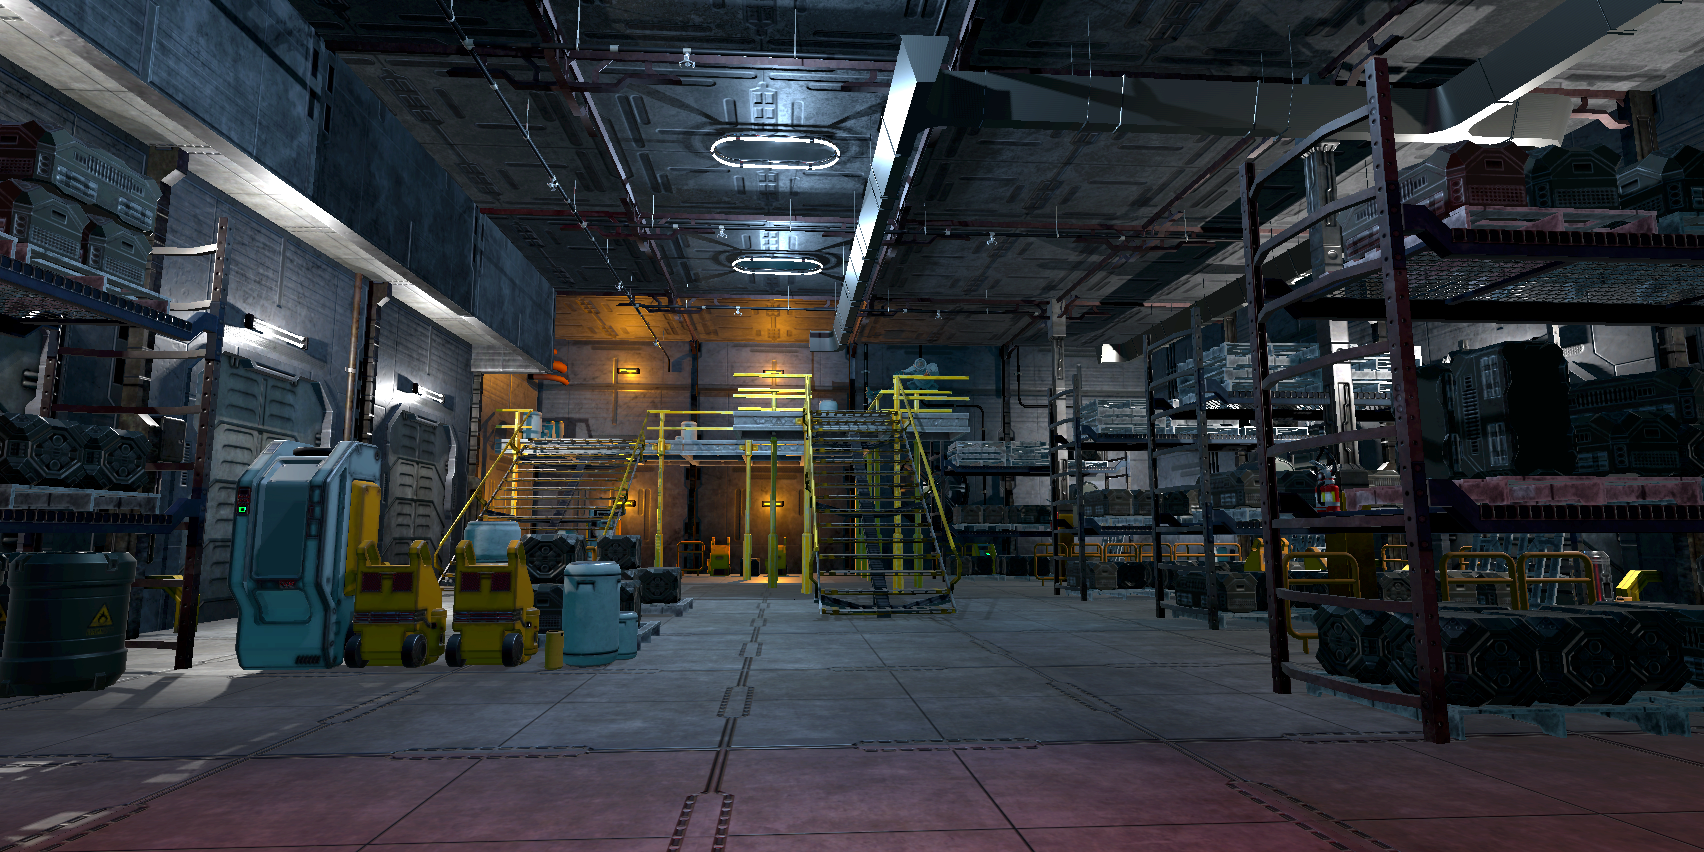
\includegraphics[width=\textwidth]{matmex-diploma-template-master/figures/tech_warehouse.png}
    \caption{Процедурно заполненное складское помещение}
    \label{fig:tech_warehouse}
    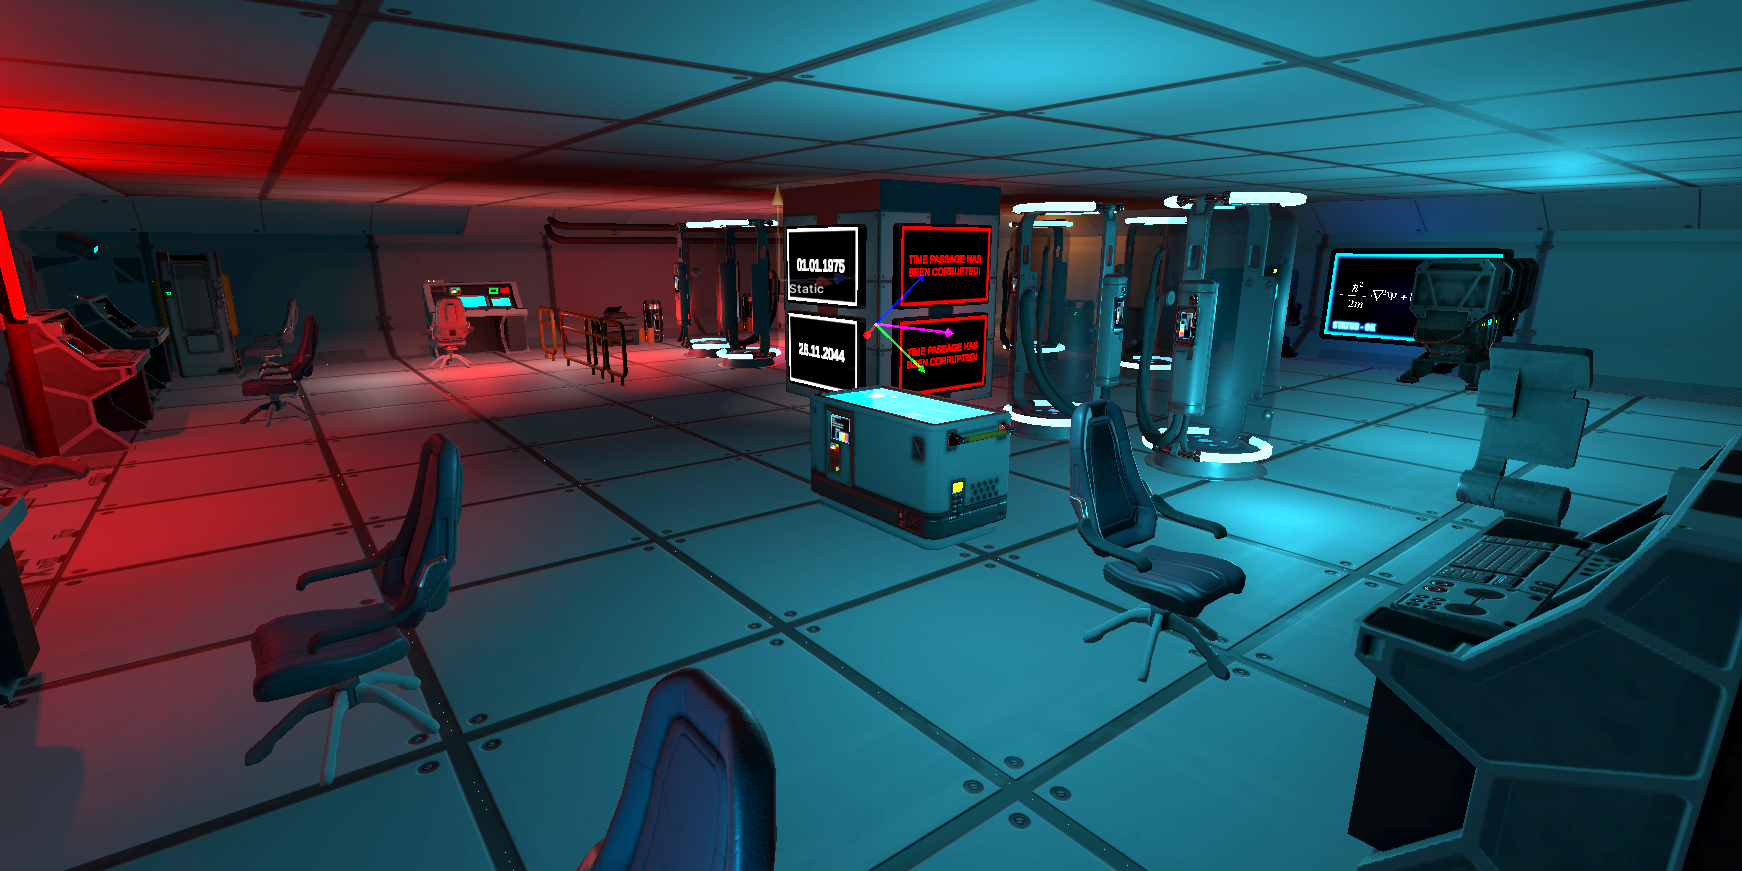
\includegraphics[width=\textwidth]{matmex-diploma-template-master/figures/laboratory.png}
    \caption{Процедурно заполненное лабораторное помещение}
    \label{fig:laboratory}
\end{figure}
% !TeX spellcheck = ru_RU
% !TEX root = vkr.tex

\section{Апробация}

Вопросы для апробационного исследования были отобраны согласно критериям методики оценки качества продукта System Usability Scale (SUS). В опросе приняли участие 13 человек. Предлагаемые формулировки и результаты исследования представлены в табл. \ref{tbl:results}.

Средний балл среди участников опроса по системе SUS составляет 68,1 при среднем показателе в 68 для систем, использующих данную систему оценивания. Все участники тестирования отметили: генератор быстро справляется с расстановкой и не создает больших задержек во времени. Полученные данные показывают, что система хорошо справляется с поставленной задачей на устройствах различных конфигураций. Более половины опрошенных не смогли с уверенностью ответить о наличии или отсутствии комнат, заполненных вручную. Такой результат может свидетельствовать о высоком уровне реалистичности игровых интерьеров.

\begin{landscape}
\begin{table}
\begin{center}
\caption{Апробационные вопросы и процент участников, выбравших предложенные варианты}
\label{tbl:results}
\rowcolors{2}{black!2}{black!10}
\scalebox{0.5}{
\begin{tabular}{|l|с|с|с|с|с|}
\hline
Вопрос &  Полностью не согласен & Скорее не согласен & Затрудняюсь ответить & Скорее согласен & Полностью согласен\\
\hline
\hline
Интерьеры комнат разнообразны.  & 0,0  & 0,0 & 0,0 & 53,9 & 46,1 \\
Комнаты выглядят пустоватыми.   & 61,5 & 15,4 & 23,1 & 0,0  & 0,0 \\
Я могу свободно перемещаться по комнатам.& 0,0 & 0,0 & 0,0 & 61,54  & 38,46 \\
Мне не нравится общее визуальное оформление комнат. & 61,5 & 30,8 & 7,7 & 0,0 & 0,0 \\
Количество реалистичных комнат превышает количество нереалистичных. & 0,0 & 0,0 & 8,3 & 25,0 & 66,7 \\
Время генерации интерьера не приемлемо. & 92,3 & 7,7 & 0,0 & 0,0 & 0,0 \\
Иерархические паттерны выдержаны хорошо. & 0,0 & 0,0 & 0,0 & 15,4 & 84,6 \\
Генератор не справляется с заполнением больших пространств. & 84,6 & 15,4 & 0,0 & 0,0 & 0,0 \\
Мебель расставлена реалистично. & 0,0 & 0,0 & 0,0 & 69,2 & 30,8 \\
Я уверен, что в игре не было заполненных вручную комнат. & 38,5 & 23,1 & 23,1 & 0,0 & 15,4 \\
\hline
\end{tabular}
}
\end{center}
\end{table}
\end{landscape}
% !TeX spellcheck = ru_RU
% !TEX root = vkr.tex

\section*{Заключение}

В рамках выполнения данной работы были получены следующие результаты.

\begin{itemize}
\item Реализованы тип-матрица и тип-вектор с использованием деревьев квадрантов в качестве метода хранения разреженных структур, а также векторно-матричные операции над ними.
\item Реализован алгоритм обхода графа в ширину с использованием линейной алгебры.
\item Реализованы параллельные версии векторно-матричных операций с помощью выражений \texttt{async} --- специальной конструкции языка F\#.
\item Выполнено экспериментальное исследование реализованного алгоритма. Обход в ширину с использованием параллельной версии матрично-векторных операций показал ускорение до 3.45 раз на матрицах среднего размера в сравнении с однопоточной версией и не показал себя эффективно на матрицах малого и большого размеров.
\end{itemize}

Результаты исследования могут иметь практическое применение в областях, где требуется анализ разреженных графовых данных. 

\setmonofont{CMU Typewriter Text}
\bibliographystyle{ugost2008ls}
\bibliography{interiors_PCG_Savelyeva_Polina}
\end{document}
